%{{{ prelude
\documentclass{beamer}
\usepackage[T1]{fontenc}
\usepackage[math]{iwona}
\usepackage{hyperref}
\usepackage{pgfpages}
\usepackage{tikz}
\usepackage{graphicx}
\usepackage{xspace}

\setbeamertemplate{navigation symbols}{}
\setbeamercolor{normal text}{bg=black,fg=white}
\setbeamercolor{alerted text}{fg=yellow}
\setbeamercolor{structure}{fg=green}

\newcommand{\titletext}{The Design and Algorithms of a Verification Condition
  Generator}
\definecolor{lightblue}{rgb}{0.5,0.5,1}
\hypersetup{colorlinks,linkcolor=lightblue,citecolor=lightblue,urlcolor=lightblue}
\hypersetup{
  pdfauthor={Radu Grigore},
  pdftitle={\titletext}}

\tikzset{statement/.style={
  rectangle,
  draw,thick,
  inner sep=2pt,minimum height=3ex}}

\title{\titletext}
\author{Radu Grigore}
\subtitle{\url{http://code.google.com/p/freeboogie}}
\date{23 August 2010}

\newcommand{\specsharp}{Spec$^\sharp$\xspace}
\def\,#1{{\lineskiplimit=0pt \oalign{\relax#1\crcr\hidewidth,\hidewidth}}}

\begin{document}
\maketitle
%{{{ plan
% Audience: Rustan and Henry.
% Principles:
%   - give a good overview
%     - spend plenty of time explaining how pieces fit together
%     - mention all the contributions explicitly
%   - go in depth into one subject (say, reachability)
% Plan
%   - motivation
%   - design and overview
%   - 
% Extra slides (for answering questions):
%   - TODO 
%}}}
%{{{ motivation
\begin{frame}
  \frametitle{program verifiers}
  \begin{block}{goals}
  \begin{itemize}
  \item
    \emph{significantly} improve the quality of programs 
    \emph{without} requiring much work from programmers
  \item 
    check \emph{automatically} that \emph{efficient} programs do
    \emph{what they should}
  \item
    easy to use, fast, \dots
  \end{itemize}
  \end{block}

  \begin{block}{guts}
  \begin{itemize}
  \item compiler-like
  \item programming language theory and algorithms
  \end{itemize}
  \end{block}
\end{frame}
%}}}
%{{{ FreeBoogie
\begin{frame}
  \begin{block}{\specsharp architecture}
  \begin{itemize}
  \item \specsharp compiler 
  \item Boogie language
  \item Boogie tool 
    \begin{itemize}
    \item \emph{verification condition generator}
    \item SMT prover
    \end{itemize}
  \end{itemize}
  \end{block}
  \begin{block}{improvements}
  \begin{itemize}
  \item \alert{configurable method}
    \begin{itemize}
    \item weakest precondition
    \item strongest postcondition
    \end{itemize}
  \item analyzes
    \begin{itemize}
    \item partial correctness
    \item \alert{reachability}
    \end{itemize}
  \item \alert{incremental}
  \end{itemize}
  \end{block}
\end{frame}
%}}}
%{{{ Boogie example
\begin{frame}
\begin{center}
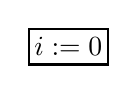
\begin{tikzpicture}
  \node[statement] (0) at (0,0) {$i:=0$};
\end{tikzpicture}
\end{center}
\end{frame}

\begin{frame}
  \frametitle{Contributions}
  \begin{itemize}
  \item semantics for core Boogie: operational, Hoare, wp, sp, relation
  \item novel use of Visitors, and the supporting tool AstGen; there's
    also a discussion of the overall design
  \item precise definition of passivation (also by Vogels, Jacobs, Pissens)
  \item study of the complexity of the passivation problem
  \item experimental comparison of wp vs sp
  \item algorithm for unsharing expression dags
  \item proof technique for algorithms that simplify verification conditions
  \item heuristic for detecting common parts of expression trees
  \item why is reachability analysis useful (in addition to correctness
    and termination)
  \item heuristics that make reachability analysis practical 
  \end{itemize}
\end{frame}
%}}}
%{{{ old
\begin{frame}
  \frametitle{Reachability Analysis for Annotated Code}
  coauthors: Mikol\'a\v{s} Janota and Micha{\l} Moskal\bigskip
  \begin{itemize}
  \item We present a general technique to catch
    \begin{itemize}
    \item \emph{dead code},
    \item bugs (or intended unsoundness) in the VC generator,
    \item inconsistent axiomatizations or specifications, and
    \item assertions that always fail (doomed code).
    \end{itemize}
  \item The technique is simple because
    \begin{itemize}
    \item we rely on a previous stage to cut loops and
    \item we use strongest postcondition (instead of wp).
    \end{itemize}
  \item The naive implementation is unusably slow, as it calls
    the prover once per program point. I sped that up to $<2$
    calls to the prover per method on average, which made it 
    usable.
  \end{itemize}
\end{frame}

\begin{frame}
  \frametitle{Edit and Verify}
  coauthor: Micha{\l} Moskal\bigskip
  \begin{itemize}
  \item Idea: If the program and specs changed a little since
    the last verification, then don't redo all the work!
  \item proof of concept implementation in Fx7
    \begin{itemize}
    \item keep the last prover query
    \item preprocess the new query, using the previous one
    \end{itemize}
  \end{itemize}
\end{frame}

\begin{frame}
  \frametitle{Strongest Postcondition of Unstructured Programs}
  coauthors: Julien Charles, Fintan Fairmichael, Joseph Kiniry
  \bigskip
  \begin{enumerate}
  \item semantics
    \begin{itemize}
    \item correctness of a flowgraph
    \item Hoare triples vs WP vs SP
    \end{itemize}
  \item algorithms
    \begin{itemize}
    \item \emph{definition of passive form}
    \item complexity of finding an optimal passive form
    \end{itemize}
  \end{enumerate}
\end{frame}

\begin{frame}
  \frametitle{FreeBoogie}
  \begin{itemize}
  \item Java clone of MSR's Boogie
  \item platform for some research
  \item status
    \begin{itemize}
    \item after a major change that is not quite finished:
      BoogiePL$\to$Boogie2
    \item main missing parts:
      \begin{itemize}
      \item invariants inference
      \item encoding Boogie2 types
      \end{itemize}
    \end{itemize}
  \item 
  \end{itemize}
\end{frame}
%}}}
%{{{ Q&A
\begin{frame}
\centerline{\Huge Q\&A}
\end{frame}
%}}}
\end{document}

